\zchapter{UCC::Events}

UCC runs a lot of events. You should go to them! Dates and times may change. 

% Event with title and date
\newenvironment{event}[3]
{
	\begin{mdframed}[backgroundcolor=white,nobreak=true]
		\color{black}{\section{#1}}
		\begin{mdframed}[backgroundcolor=white]
			When: #2
			Where: #3
		\end{mdframed}
}{
	\end{mdframed}
}

% Simpler (no boxes)
\renewenvironment{event}[3]
{
	\section{#1}
	\noindent {\bf When:} #2 \\
	{\bf Where:} #3

}{}




% By [SAS] and [GOZ]

\begin{event}{Fresher Welcome}{Friday, February 27th, 5:00PM}{Cameron Hall Loft (above the UCC clubroom)}
The Fresher welcome exists to welcome you, a new UCC member, to the club. We will have all the machines set up to play a friendly game of Wolfenstein Enemy Territory. There will be a number of current members there to talk with and get to know, and all of your questions about the club and how to use it will be answered. As a bonus, all first time members get {\bf FREE pizza}.
\end{event}

\begin{event}{Intro to Programming}{Weekly on Fridays, commencing March 6th}{UCC clubroom}
Our Introduction to Programming tutorial aims to introduce our new members to both UCC services and to basic level programming which many will find useful throughout University. This is the first part in a weekly series of talks offered by our esteemed, experienced members.
\end{event}

\begin{event}{Annual General Meeting}{Tuesday, March 10th, 1:00PM}{Guild Council Meeting Room}
The AGM is the meeting at which the new UCC Committee is elected for 2015. The only way to be represented is to attend on the day. As a Fresher, you should attend to either run for or vote for the position of the Fresher Representative, who will be your liaison for the committee. If you don't know where the Guild Council Meeting Room is, arrive at the UCC clubroom a little early to join the mass exodus.
\end{event}

\newpage

\begin{event}{Easter LAN}{Friday, 10th April, 4:00PM until the morning after}{The Loft (above UCC clubroom)}
UCC runs a number of LANs throughout the year, some with proper organisation, some without. The Easter LAN is the first big LAN of the academic year, taking place over the Easter weekend, the first weekend of mid-semester one study break. We play a number of different games, and of course you can organise your own. LANs are free for all UCC members, but you can bring a friend for around \$5 (though of course you should encourage them to join). Bring your own PCs, or use one of the limited stock in the clubroom.
\end{event}

%\begin{event}{LANs}{Throughout the Year, From Dusk til Dawn}{The Loft (above UCC clubroom)}
%The UCC hosts a number of more LANs throughout the year. As above, the Easter LAN is the first big one. Expect other LANs during the semester and breaks.
%\end{event}

\begin{event}{Cameron Hall Quiz Night}{Friday, 24th April, 6:00PM}{UWA Tavern}
Bringing together the various clubs of Cameron Hall, the quiz night is the only proper time to use your smarts throughout your degree.  (18+ Event).
\end{event}

\begin{event}{Camp}{Friday, 17th July to Monday, 20th July}{Camp Leshenaultia}
The UCC goes camping! Without tents. There is a dormitory. During the winter break, UCC will host a camp at Camp Leschenaultia. This is a chance to get your computer out of the house for a few days, tinkering and playing games with a whole bunch of other members. Don't worry, you won't be without precious internet. (18+ Event).
\end{event}

\begin{event}{41st Anniversary Dinner}{September}{TBA}
The UCC typically holds an Anniversary Dinner held sometime during our anniversary month, September, each year. Both old and new members come together to enjoy a social evening of food and drinks at a popular restaurant.
\end{event}

\begin{event}{Cameron Hall Charity Vigil}{Friday, 2nd October - during mid-semester two study break}{Cameron Hall}
Once a year, all of the clubs in Cameron Hall get together and hold a night of fun and games to raise money for charity. While the details of the night are still to come, the UCC will likely host a LAN. There will be an entry fee for this event, but expect it to be fully worth it.
\end{event}

%\begin{event}{Tech Talks}{Throughout the Year, as Interest Demands}{UCC clubroom and/or the Loft}
%A chance to demonstrate your own tech-y knowledge, or learn from someone else. Previous topics include: ``Introduction to TOR''; and ``The Magic of Data Compression''. %Early on in the semester, a number of tech talks will cover learning to use the club's machines.
%\end{event}

%\begin{mdframed}[backgroundcolor=white]
\color{black}{\section{FUCC Camp Scholarship}\label{camp_scholarship}}
\noindent \color{black}{\bf Incoming message from James Cox and Lionel Price:}


\noindent \color{black}{For new members to UCC, Lionel and I would like to tell you about our
full-ride scholarship program. We realise that Camp is fairly
expensive, but as once-freshers made good we are financially able to
provide unto others. Previous recipients of these scholarships have
gone onto great things so we are proud to offer it once more in 2015.
I would encourage everyone who is interested to take advantage of this
offer - I had a great time my first UCC Camp which is part of the
reason why I now offer this scholarship.

Two first-time UCC Campers will have their entry fee paid for by us.
As before, you will also obtain the privilege, if you should so wish,
to add a pink \textcolor{black}{F} to your UCC tags, denoting sophistication, intellect,
and exclusive membership of an elite group of teamkilling imbeciles.

To be eligible for this award, you must be a UWA student, member of
UCC, and to not have attended a previous UCC Camp. Applicants will
also need to declare in writing that they will participate in at least
one game of DotA during UCC Camp, and that when we play ET you will
not be a noob in the back with a mortar accomplishing nothing all
match.}
\begin{comment}
\begin{figure}[H]
	\centering
	
\includegraphics[width=0.5\textwidth]{figures/WolfET_logo.jpg}
	\caption{ET Logo. Don't be a noob.}
\end{figure}

%\end{mdframed}

%\begin{figure}[H]
%	\centering
%	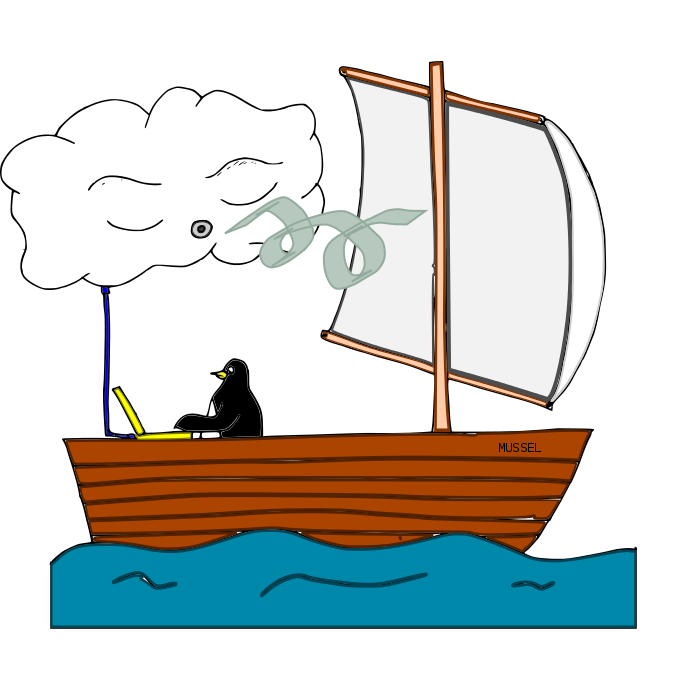
\includegraphics[width=0.8\textwidth]{figures/tux_boat.png}
%	\caption{Tux enjoys Lake Leshenaultia at UCC::Camp \\ (Please note: There will not actually be watersports at the camp)}
%	\label{tux_boat.png}
%\end{figure}
\end{comment}
